\section{Modellistica ed equazioni differenziali lineari}
% TODO:
% • Cenni di modellistica (circuiti elettrici e sistemi
% meccanici)
% • L’equazione differenziale lineare a coefficienti
% costanti quale modello di un sistema dinamico
% scalare



\subsection{Cenni di modellistica}

La modellistica è la costruzione di modelli matematici dei sistemi a partire dalle leggi fondamentali o dai dati sperimentiali.

\subsubsection{Circuiti elettrici - Resistenza}

\begin{figure}[!ht]
	\centering
	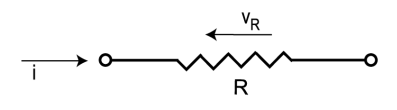
\includegraphics[width=0.3\columnwidth]{./images/resistenza.png}
	\caption{Resistenza}
	\label{fig:resistenza}
\end{figure}

\begin{align}
	V_R = R \cdot I
\end{align}


\subsubsection{Circuiti elettrici - Induttanza}

\begin{figure}[!ht]
	\centering
	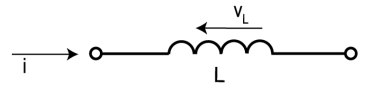
\includegraphics[width=0.3\columnwidth]{./images/induttanza.png}
	\caption{Induttanza}
	\label{fig:induttanza}
\end{figure}

\begin{align}
	V_L = L \cdot \frac{dI}{dt} = L \cdot DI
\end{align}


\subsubsection{Circuiti elettrici - Capacità}

\begin{figure}[!ht]
	\centering
	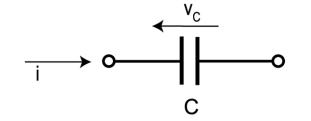
\includegraphics[width=0.3\columnwidth]{./images/capacita.png}
	\caption{Capacità}
	\label{fig:capacita}
\end{figure}

\begin{align}
	V_C = \frac{Q}{C} = \frac{1}{C} \int_{-\infty}^{t} i(\tau) d\tau \Rightarrow DV_C = \frac{I}{C}
\end{align}

\subsubsection{Sistemi meccanici - Massa}
\begin{figure}[!ht]
	\centering
	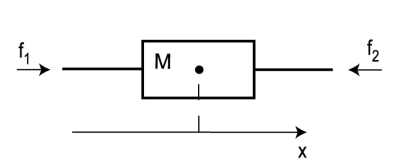
\includegraphics[width=0.3\columnwidth]{./images/massa.png}
	\caption{Massa}
  \label{fig:massa}
\end{figure}

\begin{align}
	MD^2 x(t) = f_1(t) - f_2(t)
\end{align}

\subsubsection{Sistemi meccanici - Molla}
\begin{figure}[!ht]
	\centering
	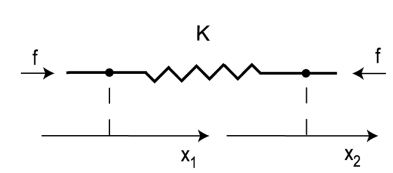
\includegraphics[width=0.3\columnwidth]{./images/molla.png}
	\caption{Molla}
  \label{fig:molla}
\end{figure}

\begin{align}
	f(t) = K(x_1(t) - x_2(t))
\end{align}


\subsubsection{Sistemi meccanici - Ammortizzatore}
\begin{figure}[!ht]
	\centering
	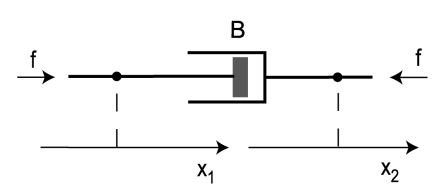
\includegraphics[width=0.3\columnwidth]{./images/ammortizzatore.png}
	\caption{Ammortizzatore}
	  \label{fig:ammortizzatore}
\end{figure}

\begin{align}
	f(t) &= B(v_1(t) - v_2(t)) \\
  &= BD(x_1(t) - x_2(t))
\end{align}




\subsection{Equazioni differenziali lineari}
Avendo un sistema di equazioni differenziali lineari a coefficienti costanti:
\begin{align}
  \sum_{i=0}^{n} a_i D^i y = \sum_{i=0}^{m} b_i D^i u
\end{align}


Si noti che:
\begin{itemize}
  \item $n$ è l'ordine dell'equazione differenziale se $n \geq m$
  \item $\rho = n - m$ è l'ordine relativo del sistema se $n \geq m$
\end{itemize}

\subsubsection{Proprietà}

Il sistema $\sum$ è lineare e stazionario.


